% filepath: /rds/general/user/moa324/home/projects/cyberwheel/research_docs/poster/adaptive_deception_poster.tex
\documentclass[landscape]{ImperialPoster}

% Define poster info
\postertitle{AI-Driven Cyber Defense: 89\% Better Protection Through Adaptive Deception}
\posterauthors{Miracle Akanmode \quad Supervisor: Kelly Zhang}

% Key macros for consistent data presentation
\newcommand{\pporeward}{309.1}
\newcommand{\staticreward}{163.8}
\newcommand{\rulereward}{79.2}
\newcommand{\inactive}{-1.6}
\newcommand{\decoyrate}{73.2\%}
\newcommand{\protectrate}{82.4\%}
\newcommand{\alertignored}{67\%}
\newcommand{\latencyppo}{2.3}

% Required packages
\usepackage{multicol}
\usepackage{amsmath,amssymb}
\usepackage{booktabs}
\usepackage{tikz}
\usepackage{pgfplots}
\pgfplotsset{compat=1.18}  % Use latest version or specify 1.16/1.17 if needed
\usetikzlibrary{positioning,shapes,arrows,fit,calc,backgrounds}
% Set proper colors for Imperial template
\definecolor{ICLBlue}{RGB}{0,62,116}

% Fix figure spacing
\setlength{\intextsep}{0.5em} % Space above/below in-text figures
\setlength{\textfloatsep}{0.5em} % Space between floats and text

% Define custom accent colors
\definecolor{cwDecoy}{RGB}{243,156,18}
\definecolor{cwAlert}{RGB}{231,76,60}
\definecolor{cwFlow}{RGB}{52,152,219}




\begin{document}
\titlesection

\medskip % Vertical whitespace

\begin{multicols}{4} % Four-column layout per Imperial template

% COLUMN 1
\section{The Cyber Challenge}
\begin{itemize}
\item \textbf{Asymmetric Advantage}: Attackers need to find just one vulnerability; defenders must protect everything
\item \textbf{Alert Fatigue}: \alertignored{} of alerts ignored due to volume
\item \textbf{Base-Rate Fallacy}: Most alerts are false positives, causing real threats to be missed
\item \textbf{Static Defenses Fail}: Predictable patterns exploited by attackers
\end{itemize}

\begin{figure}[H]
\centering
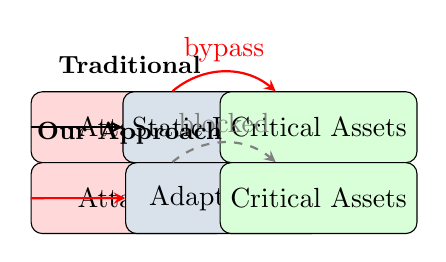
\begin{tikzpicture}[
    scale=0.3,
    box/.style={rectangle,draw,rounded corners,minimum width=2.5cm,minimum height=0.9cm},
    redbox/.style={box,fill=red!15},
    bluebox/.style={box,fill=ICLBlue!15},
    greenbox/.style={box,fill=green!15},
    arrow/.style={->,>=stealth,thick}
]
% Traditional approach
\node[redbox] (attack) at (0,0) {Attacker};
\node[bluebox] (static) at (4,0) {Static Defenses};
\node[greenbox] (assets) at (8,0) {Critical Assets};

\draw[arrow] (attack) -- (static);
\draw[arrow, red, thick] (attack) to[bend left=40] node[above] {bypass} (assets);

% Our approach
\node[redbox] (attack2) at (0,-3) {Attacker};
\node[bluebox] (adaptive) at (4,-3) {Adaptive AI};
\node[greenbox] (assets2) at (8,-3) {Critical Assets};

\draw[arrow, red] (attack2) -- (adaptive);
\draw[arrow, dashed, gray] (attack2) to[bend left=40] node[above] {blocked} (assets2);

\node[above=0.1cm of attack, font=\small\bfseries] {Traditional};
\node[above=0.1cm of attack2, font=\small\bfseries] {Our Approach};
\end{tikzpicture}
\caption{Static vs. adaptive RL approach.}
\end{figure}

\begin{quote}
"Traditional defenses remain static while attackers continuously adapt. An intelligent defense must adapt as quickly as the threat."
\end{quote}

\section{Research Aim}
To develop and evaluate an RL Agent that learns optimal decoy placement strategies, maximizing attacker deception while minimizing defensive resource costs.

\textbf{Research Questions:}
\begin{enumerate}
\item Can RL effectively learn adaptive decoy deployment?
\item How does a learned approach compare to traditional methods?
\item What strategic behaviors emerge and how do they scale?
\end{enumerate}

\columnbreak

% COLUMN 2
\section{Method}

\begin{figure}[H]
\centering
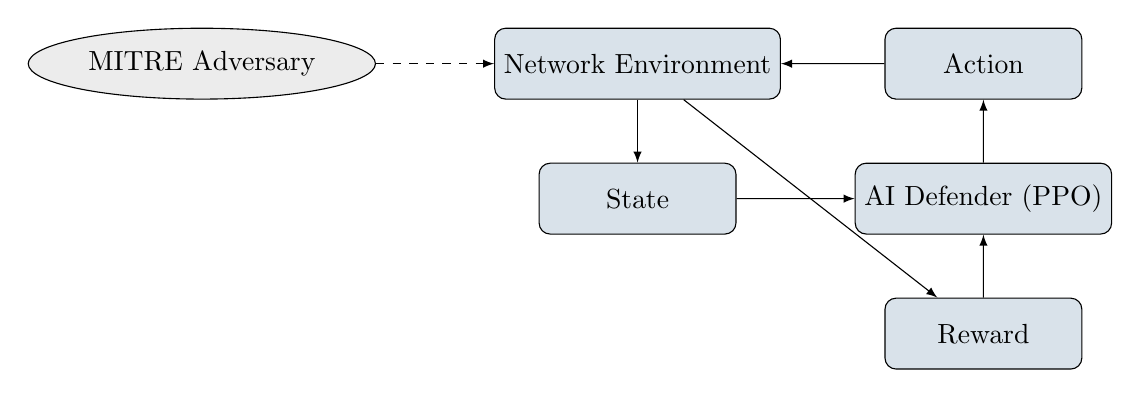
\begin{tikzpicture}[
    scale=0.3,
    block/.style={rectangle, draw, rounded corners, minimum width=2.5cm, minimum height=0.9cm, text centered, fill=ICLBlue!15},
    line/.style={draw, ->, >=latex},
    cloud/.style={draw, ellipse, minimum width=2cm, minimum height=0.9cm, text centered, fill=gray!15}
]
% Place nodes
\node [block] (env) {Network Environment};
\node [block, below=0.8cm of env] (state) {State};
\node [block, right=1.5cm of state] (agent) {AI Defender (PPO)};
\node [block, above=0.8cm of agent] (action) {Action};
\node [block, below=0.8cm of agent] (reward) {Reward};
\node [cloud, left=1.5cm of env] (attacker) {MITRE Adversary};

% Draw edges
\draw [line] (env) -- (state);
\draw [line] (state) -- (agent);
\draw [line] (agent) -- (action);
\draw [line] (action) -- (env);
\draw [line] (env) -- (reward);
\draw [line] (reward) -- (agent);
\draw [line, dashed] (attacker) -- (env);
\end{tikzpicture}
\caption{Reinforcement learning approach.}
\end{figure}

\textbf{Environment:}
\begin{itemize}
\item Multi-subnet enterprise network (15-200 hosts)
\item Fixed attacker following MITRE ATT\&CK tactics
\item Decoys can be deployed or removed in any subnet
\end{itemize}

\textbf{Reward Structure:}
$\begin{aligned}
R_t &= 10 v_r \mathbf{1}[\text{decoy hit}] \\
    &- v_r \mathbf{1}[\text{asset hit}] \\
    &- 20\mathbf{1}[\text{deploy}] - \mathbf{1}[\text{remove}]
\end{aligned}$

\smalltext{where $v_r$ escalates with attack progression (recon → impact) and costs penalize excessive deployment}

\begin{figure}[H]
\centering
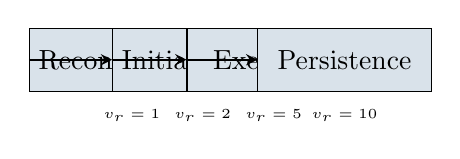
\begin{tikzpicture}[
    scale=0.3,
    box/.style={rectangle,draw,fill=ICLBlue!15,minimum width=2.2cm,minimum height=0.8cm},
    arrow/.style={thick,->,>=stealth}
]
\node[box] (recon) at (0,0) {Reconnaissance};
\node[box] (initial) at (3,0) {Initial Access};
\node[box] (execution) at (6,0) {Execution};
\node[box] (persistence) at (9,0) {Persistence};

\draw[arrow] (recon) -- (initial);
\draw[arrow] (initial) -- (execution);
\draw[arrow] (execution) -- (persistence);

\node[below=0.1cm of recon, font=\tiny] {$v_r=1$};
\node[below=0.1cm of initial, font=\tiny] {$v_r=2$};
\node[below=0.1cm of execution, font=\tiny] {$v_r=5$};
\node[below=0.1cm of persistence, font=\tiny] {$v_r=10$};
\end{tikzpicture}
\caption{MITRE ATT\&CK-based attack progression.}
\end{figure}

\textbf{Comparison Baselines:}
\begin{itemize}
\item \textbf{Static}: Fixed interval placement with capacity limits
\item \textbf{Rule-based}: Temporal heuristics
\item \textbf{Inactive}: No decoys (control)
\end{itemize}

\columnbreak

% COLUMN 3
\section{Results}

\largepercent{89\%}
Improvement in defensive effectiveness

\begin{figure}[H]
\centering
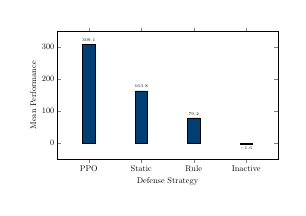
\begin{tikzpicture}[scale=0.3]
\begin{axis}[
    ybar,
    bar width=15pt,
    xlabel={Defense Strategy},
    ylabel={Mean Performance},
    symbolic x coords={PPO,Static,Rule,Inactive},
    xtick=data,
    ymin=-50,
    ymax=350,
    width=0.9\linewidth,
    height=7cm,
    nodes near coords,
    nodes near coords align={vertical},
    every node near coord/.append style={font=\tiny},
    enlarge x limits=0.2
]
\addplot[fill=ICLBlue] coordinates {(PPO,\pporeward) (Static,\staticreward) (Rule,\rulereward) (Inactive,\inactive)};
\end{axis}
\end{tikzpicture}
\caption{Performance comparison across strategies.}
\end{figure}

\begin{table}[H]
\caption{Security metrics comparison.}
\small
\begin{tabular}{L{0.24\linewidth} C{0.18\linewidth} C{0.18\linewidth} C{0.18\linewidth}}
\toprule
Metric & PPO & Static & Rule\\
\midrule
Deception & \decoyrate & 45.1\% & 32.4\% \\
Protection & \protectrate & 61.7\% & 48.2\% \\
Latency & \latencyppo & 4.1 & 5.8 \\
\bottomrule
\end{tabular}
\end{table}

\section{Strategic Behavior}

\begin{figure}[H]
\centering
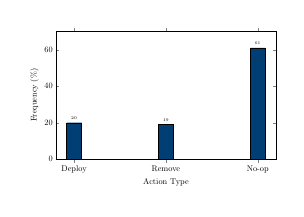
\begin{tikzpicture}[scale=0.3]
\begin{axis}[
    ybar,
    bar width=18pt,
    xlabel={Action Type},
    ylabel={Frequency (\%)},
    symbolic x coords={Deploy,Remove,No-op},
    xtick=data,
    ymin=0,
    ymax=70,
    width=0.9\linewidth,
    height=7cm,
    nodes near coords,
    nodes near coords align={vertical},
    every node near coord/.append style={font=\tiny}
]
\addplot[fill=ICLBlue] coordinates {(Deploy,20) (Remove,19) (No-op,61)};
\end{axis}
\end{tikzpicture}
\caption{Action distribution showing strategic restraint.}
\end{figure}

\boldsection{Emergent Intelligence:} The AI learned that excessive decoy deployment is counterproductive - it increases costs without proportional security gains. This strategic restraint emerged naturally.

\columnbreak

% COLUMN 4
\section{Network Visualization}
\begin{figure}[H]
\centering
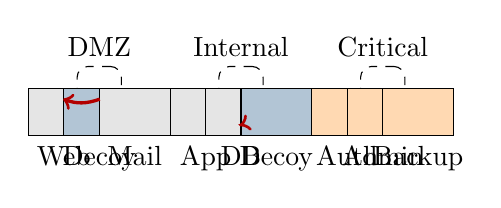
\begin{tikzpicture}[
    scale=0.3,
    server/.style={rectangle,draw,minimum width=0.9cm,minimum height=0.6cm,fill=gray!20},
    decoy/.style={rectangle,draw,minimum width=0.9cm,minimum height=0.6cm,fill=ICLBlue!30},
    asset/.style={rectangle,draw,minimum width=0.9cm,minimum height=0.6cm,fill=orange!30},
    attack/.style={->,very thick,red!70!black},
    subnet/.style={rectangle,rounded corners,draw,dashed,inner sep=8pt}
]
% Subnets
\node[subnet,label=above:DMZ] (dmz) at (0,0) {};
\node[subnet,label=above:Internal] (int) at (6,0) {};
\node[subnet,label=above:Critical] (crit) at (12,0) {};

% Servers DMZ
\node[server,label=below:Web] (web) at (-1.5,-1) {};
\node[decoy,label=below:Decoy] (dec1) at (0,-1) {};
\node[server,label=below:Mail] (mail) at (1.5,-1) {};

% Servers Internal
\node[server,label=below:App] (app1) at (4.5,-1) {};
\node[server,label=below:DB] (app2) at (6,-1) {};
\node[decoy,label=below:Decoy] (dec2) at (7.5,-1) {};

% Servers Critical
\node[asset,label=below:Auth] (db) at (10.5,-1) {};
\node[asset,label=below:Admin] (auth) at (12,-1) {};
\node[asset,label=below:Backup] (admin) at (13.5,-1) {};

% Attack paths
\draw[attack] (web) to[bend left=20] (dec1);
\draw[attack] (app1) to[bend right=20] (dec2);
\end{tikzpicture}
\caption{Network with AI-placed decoys intercepting attacks.}
\end{figure}

\section{Scaling Performance}
\begin{table}[H]
\caption{Performance across network sizes.}
\small
\begin{tabular}{L{0.24\linewidth} C{0.24\linewidth} R{0.24\linewidth}}
\toprule
Network & Reward & Retention\\
\midrule
15 hosts & 309.1 & 100\% \\
50 hosts & 325.4 & 105\% \\
200 hosts & 298.2 & 96\% \\
\bottomrule
\end{tabular}
\end{table}

\section{Conclusion}

\textbf{Key Findings:}
\begin{itemize}
\item AI successfully learns adaptive cyber defense strategies
\item 89\% improvement over traditional approaches
\item Strategic restraint emerges naturally 
\item Performance scales to enterprise networks
\end{itemize}

\smalltext{Statistical validation: 5 seeds, 95\% confidence intervals, ANOVA $p<0.001$}

\section{Future Work}
\begin{itemize}
\item Adversarial co-evolution (self-play)
\item Multi-objective optimization 
\item Real-world testing with human red teams
\item Transfer learning across network topologies
\end{itemize}

\section{Contact \& References}
\smalltext{
\textbf{Miracle Akanmode} \quad Supervisor: Kelly Zhang\\
\textbf{Email}: miracle.akanmode24@imperial.ac.uk\\
\textbf{References}: Sommer \& Paxson (Base-rate fallacy), Schulman et al. (PPO), MITRE ATT\&CK Framework
}

\end{multicols}
\end{document}